\chapter{Introduction}

The review of published literature reveals that fluid-elastic galloping has a potential to be used as a mechanism for energy extraction \citep{Barrero-Gil2010a}. Thus, the following questions emerged. What are the optimum parameters for energy transfer in a galloping system? How do they influence galloping?

Over the years, VIV has been the popular research problem  studied on flow induced vibrations. As a result, the parameters used to describe VIV problems (i.e \mstar, $\zeta$ and \ustar) have been incorporated to describe galloping, which could be observed throughout the current literature \citep{Barrero-Gil2009,Barrero-Gil2010a,Parkinson1964}.

However, mean power data presented using this classical VIV parameters \citep{Barrero-Gil2010a}, does not provide a good collapse. A potential reason for this could be the difference in time scales of VIV and galloping.

Therefore, more relevant governing parameters for galloping could be obtained using the relevant time scales, from which, the optimum power output could be obtained. The work presented in this chapter is focused on testing this hypothesis. 

Since the main mathematical model used to describe galloping is the Quasi-steady state model, the fluid-dynamic characteristics of flow over a static body are presented and discussed first. Then, the natural time scales of the system are obtained using the linearised QSS model. Next, the new non-dimensional governing parameters  \massstiff\ and \massdamp, are formulated by non-dimensionalising the QSS model from these natural time scales, followed by a comparison of galloping data using the classical VIV parameters and  \massstiff\ and \massdamp. Then, the influence of \massstiff \ and \massdamp \ and the conditions for an optimum power output are discussed from QSS data. Finally, the QSS data are compared and discussed against FSI direct numerical simulations and final conclusions are presented.

\clearpage

\subsection{Static body results}

The main data acquisition tool for galloping is the QSS model. As discussed in chapter \label{sec:QSS_model_methodology}, the QSS model uses an interpolation polynomial of the static body lift data as the driving force of the QSS equation. These static body data and the polynomial data are presented here.  Figure \ref{fig:lift_curves} shows the plots of $C_y$ as a function of $\theta$, as well as the interpolation polynomial curves. Data are acquired for high and low Reynolds numbers. For high Reynolds numbers, the static body polynomial data are obtained from \cite{Parkinson1964} while for low Reynolds numbers a $7^{th}$ order non-linear least square regression fit on static body DNS simulations were used. The coefficients of these  polynomials are presented in table \ref{table:cy-coefficients}.


\begin{figure}

  \setlength{\unitlength}{\textwidth}
  \begin{picture}(1,0.25)(0,0.8)
  
    % % %90
      \put(0.025,0.81){\includegraphics[width=0.5\unitlength]{./chapter-pi_1_pi_2/FnP/gnuplot/lift_curve_200.eps}}
      \put(0.495,0.81){\includegraphics[width=0.5\unitlength]{./chapter-pi_1_pi_2/FnP/gnuplot/lift_curve_park.eps}}
 	\put(0.02,0.93){ \large $C_y$} 	
% 	\put(0.56,1.02){ $\theta$}
 	
        \put(0.25,0.8){ $\theta$} 	
        \put(0.75,0.8){ $\theta$}
        
        \put(0.117,1.01){(a)}
        \put(0.565,1.01){(b)}
      \end{picture}

  \caption{Lift coefficient, $C_y$, as a function of incidence angle $\theta$, for a static square cross section. (a) Data from simulations at $Re=200$  (b) data from \cite{Parkinson1964} at $Re=22300$. Points ($\bullet$) are measurements from the simulations. At $\reynoldsnumber=200$. Curves in both plots are 7th-order interpolating polynomials used to predict the fluid forcing for the QSS model. $C_y$ is the force coefficient of the force which occurs normal to the induced velocity.}
    \label{fig:lift_curves}
\end{figure}


\begin{table}[ht]

\begin{center}
\setlength{\unitlength}{\textwidth}

\begin{tabular}{c c c c c} % centered columns (4 columns)
\hline\hline %inserts double horizontal lines
\\[0.2ex]
Case & $a_1$ & $a_3$ & $a_5$ & $a_7$ \\ [0.8ex] % inserts table 
%heading
\hline 
\\[0.8ex]% inserts single horizontal line
Re=200 & 2.32 & 197.8 & 4301.7 & 30311.9 \\[0.8ex]% inserting body of the table
Re=22300 & 2.69 & 168 & 1670 & 59900 \\ [1ex] % [1ex] adds vertical space
\hline %inserts single line
\end{tabular}

\caption{Coefficient values used in the 7th order interpolation polynomial for high ($Re=22300$) and low ($Re=200$) Reynolds numbers. These data are used as input data to calculate the right-hand side of Eq. \ref{final_equation_motion} throughout this study.}
 
\label{table:cy-coefficients} % is used to refer this table in the text
\end{center}
\end{table}



There are several differences that can be observed between high and low Reynolds number data. The peak value of $C_y$ is  significantly lower at $\reynoldsnumber=200$ ($C_y=0.12$ at $5^\circ$) compared to $\reynoldsnumber=22300$ ($C_y=0.57$ at $13^\circ$) . The inflection point present around $8^\circ$ for $\reynoldsnumber=22300$ is not present at $\reynoldsnumber=200$. This agrees with the findings of \cite{Luo2003}. \cite{Luo2003} concluded that hysteresis in the system response occurs due to the inflection point in the $C_y$ curve. Therefore, hysteresis could not be observed at $\reynoldsnumber=200$.

The range of incident flow angles where $C_y$ remains positive is narrow at $\reynoldsnumber=200$ ($0^\circ <\theta \leq$ $7^\circ$) compared to $\reynoldsnumber=22300$ ($0^\circ <\theta \leq 15^\circ$). This positive range sustains galloping, as the power is only transferred from the fluid to the supporting structure within this range of incident angles. This is because the fluid forces are acting in the 
direction of velocity of the body, or in phase with, the oscillating body as demonstrated by equation \ref{eqn:power_alt}. Incident angles beyond this range suppress the galloping as power is transferred in the opposite direction, i.e; from body to fluid. Thus, it is expected that the transferred power at $\reynoldsnumber=200$ to be significantly lower than at $\reynoldsnumber=22300$, because of the relative low values of $C_y$ and the narrow range of positive $C_y$ at $\reynoldsnumber=200$.

\section{Formulation of the non-dimensionalised parameters \massstiff \ and \massdamp }
\label{sec: pi_1,pi_2_formulation}


The natural time scales of the system could be obtained by linearising the quasi-steady equation of motion, (Eq:\ref{final_equation_motion}) and finding the eigenvalues. The non-linear terms of the forcing function are truncated and the equation of motion could be expressed as, 

\begin{equation}
	\label{eqn:eom_linear}
	m\ddot{y}{+}c\dot{y}{+}ky{=}\frac{1}{2}\rho U^2 \mathcal{A} a_1\left(\frac{\dot{y}}{U}\right),
\end{equation}

After combining the $\dot{y}$ terms and solving for eigenvalues the following solutions for the eigenvalues could be obtained. 

\begin{equation}
	\label{eqn:eigs}
	\lambda_{1,2}= -\frac{1}{2}\frac{c-\frac{1}{2}\rho U\mathcal{A}a_1}{m}\pm\frac{1}{2}\sqrt{\left[\frac{c-\frac{1}{2}\rho U\mathcal{A}a_1}{(m)}\right]^2-4\frac{k}{m}}.
\end{equation} 

Galloping essentially occurs at low frequencies therefore it can be assumed that the spring is relevantly weak and therefore, $k \rightarrow 0$. Hence a single non-zero eigenvalue remains which is, 

\begin{equation}
	\label{eqn:eigs_nospring}
	\lambda=-\frac{c-\frac{1}{2}\rho U\mathcal{A}a_1}{m}.
\end{equation}

Further, if it is assumed that the mechanical damping is weaker than the fluid dynamic forces on the body, therefore the non zero eigenvalue could be further simplified to,

\begin{equation}
	\label{eqn:eigs_nospring_nodamp}
	\lambda=\frac{\frac{1}{2}\rho U\mathcal{A}a_1}{m}.
\end{equation}  

In this representation $\lambda$ represents the inverse time scale of the motion of the body due to the effect of long-time fluid dynamic forces (or forced due to the induced velocity). This term could also be re-written and $\lambda$ could be expressed as 

\begin{equation}
	\label{eqn:timescale}
	\lambda = \frac{a_1}{m^*}\frac{U}{D}
\end{equation}

This form clearly shows the significant parameters that influence the inverse time scale of the system. $\partial C_Y / \partial \alpha $, the rate of change in the fluid dynamic force on the body, with respect to the induced angle of attack, is represented by $a_1$. $\frac{U}{D}$ represents the inverse advective time scale of the incoming flow, and the mass ratio is represented by \mstar. Increasing $a_1$ would result in a rapid change of the fluid dynamic force with a small change of the induced angle $\theta$, which is proportional to transverse velocity $\dot{y}$. It can be seen in equation \ref{eqn:timescale} that an increase of $a_{1}$ would result in an increase of the inverse time scale or decrease the response time of the body. In contrast the mass ratio has the opposite effect where an increase in \mstar will lead to a decrease in $\lambda$, since a heavier body (or a body with higher inertia) would have a slower response. 

In order to find the relevant dimensionless groups of the problem, the time scale formulated could be used to non-dimensionalise the equation of motion. The equation of motion presented in Equation \ref{final_equation_motion} can be non-dimensionalised using the non dimensional time $\tau$, defined as $\tau=t(a_1/m^*)(U/D)$. The non-dimensional equation of motion could then be represented as, 

\begin{equation}
	\label{eqn:eom_nondim}
	\ddot{Y} + \frac{m^{*2}}{a_1^2}\frac{kD^2}{mU^2}Y = \left(\frac{1}{2} - \frac{m^*}{a_1}\frac{cD}{mU}\right)\dot{Y} - \frac{a_1A_3}{m^{*2}}\dot{Y}^3 + \frac{a_1^3a_5}{m^{*4}}\dot{Y}^5 - \frac{a_1^5a_7}{m^{*6}}\dot{Y}^7.
\end{equation}

The equation could be further altered by regrouping the coefficients into non-dimenasional groups and could be expressed as, 

\begin{equation}
	\label{eqn:eom_nondim_regroup}
	\ddot{Y} + \frac{4\pi^{2}m^{*2}}{U^{*2}a_1^2}Y = \left(\frac{1}{2} - \frac{c^*m^*}{a_1}\right)\dot{Y} - \frac{a_1A_3}{m^{*2}}\dot{Y}^3 + \frac{a_1^3a_5}{m^{*4}}\dot{Y}^5 - \frac{a_1^5a_7}{m^{*6}}\dot{Y}^7,
\end{equation}  

\ustar is the reduced velocity which is the typical independent variable used in vortex-induced vibration studies. \cstar is the non-dimensional damping parameter which is expressed as $c^*=cD/mU$. 

By analysing equation \ref{eqn:eom_nondim_regroup} it is clear that five dimensionless parameters play a role in setting the response of the system. These are namely the stiffness, damping, mass ratio, the geometry and the Reynolds number. The stiffness is represented by the reduced velocity \ustar, the damping by \cstar and the mass ratio by \mstar. The geometry and the Reynolds number are represented by the coefficients $a_n$, of the polynomial fit to the $C_y$ curve. Using the natural time scales of the system, grouping of these non-dimensional parameters into two groups in the non-dimensional equation of motion, suggests that there are two groups that govern the response which are: $\Gamma_1 = 4\pi^2m^{*2}/U^{*2}a_1^2$ and $\Gamma_2 = c^*m^*/a_1$. $\Gamma_1$ could be described as a combined mass-stiffness, where $\Gamma_2$ could be expressed as a combined mass-damping parameter for a given geometry and a Reynolds number. It is assumed that the stiffness plays a minor role, $\Gamma_2$ seems more likely parameter to collapse the data. The wind tunnel data in the classic paper of galloping by \citet{Parkinson1964} adopted a parameter similar to $\Gamma_2$ to collapse the data. 

All of the quantities that formulate $\Gamma_1$ and $\Gamma_2$ except $a_1$ in theory, could be obtained before an experiment. However in order to obtain the value of $a_1$, static body experiments are required making it relatively difficult to obtain. Here, the Reynolds number and the geometry remains constant and therefore multiplying $\Gamma_1$ by ${a_1}^2$ and $\Gamma_2$ by $a_1$ suitable parameters could be obtained, and formulate a mass-stiffness parameter $\massstiff =  4\pi^2m^{*2}/U^{*2}$, and a mass-damping parameter defined as $\massdamp = c^*m^*$ could be formulated. Therefore equation \ref{eqn:eom_nondim_regroup} can be written in terms of \massstiff \ and \massdamp. 

\begin{equation}
	\label{eqn:eom_nondim_regroup_pi_1_pi_2}
	\ddot{Y} + \massstiff Y = \massdamp \dot{Y} - \frac{a_1a_3}{m^{*2}}\dot{Y}^3 + \frac{a_1^3a_5}{m^{*4}}\dot{Y}^5 - \frac{a_1^5a_7}{m^{*6}}\dot{Y}^7,
\end{equation} 

From equation \ref{eqn:eom_nondim_regroup_pi_1_pi_2}, it is clear that the governing parameters of the non dimensionlised equation are \massstiff \ \massdamp\ and \mstar. However, from closer inspection it is possible to see that \mstar\ has an impact on the non-linear terms of the forcing function. The velocity of the body and hence the induced angle of attack needs to be very high in order for the non-linear terms to be applicable. 









